\section{LoRaWAN}
  
\begin{frame}[fragile]
  \frametitle{A deeper look at LoRa}
  \begin{itemize}
      \item LoRaWAN is a Low Power Wide Area Network (LPWAN) specification intended for wireless battery operated Things in regional, national or global network. 
      \item LoRaWAN target key requirements of internet of things:
      \begin{itemize}
      	\item secure bi-directional communication
      	\item mobility
      	\item localization services 
      \end{itemize}
  \end{itemize}
\end{frame}

\begin{frame}[fragile]
  \frametitle{LoRa devices sync}
  For time synchronization gateways periodically broadcast so-called beacons. Each beacon
  minimally contains:
  \begin{itemize}
      \item available channels (ChMask)
      \item current GPS time (Time)
      \end{itemize}
      The broadcasting of beacons (in implicit mode) is done time-synchronously (BEACON\_INTERVAL) by all gateways of a network with no interference.
      \begin{figure}
  \centering
  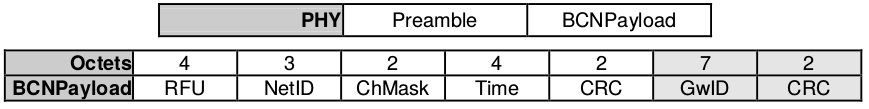
\includegraphics[width=\textwidth]{img/lora_beaconing.png}
  \end{figure}
\end{frame}

\begin{frame}[fragile]
  \frametitle{LoRa MAC Payload Frame}
  
 \begin{figure}
  \centering
  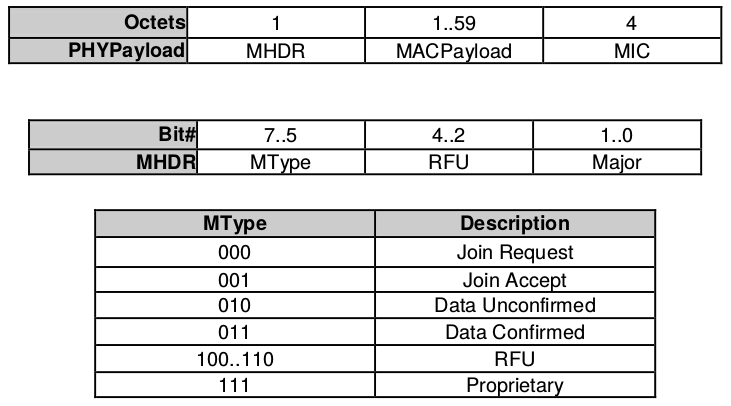
\includegraphics[width=\textwidth]{img/mac_frame.png}
  \end{figure}

\end{frame}


\begin{frame}[fragile]
  \frametitle{LoRaWAN Classes}
  \begin{figure}
    \centering
    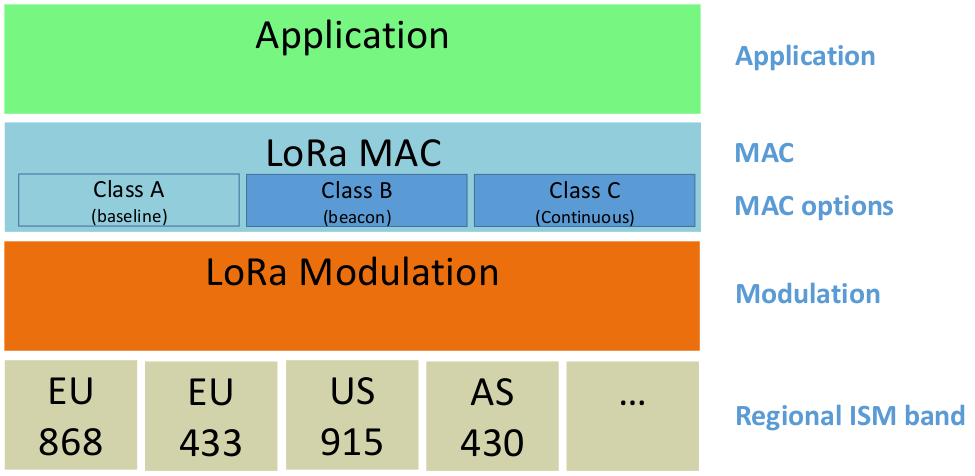
\includegraphics[width=0.9\textwidth]{img/loraClasses.png}
  \end{figure}
\end{frame}


\begin{frame}[fragile]
  \frametitle{Class A end-devices}
  \begin{itemize}
    \item Its funtionalities are implemented by every end-device.
    \item Uplink: devices transmit following Aloha method.
    \item Downlink: after a transmission two tiny time windows are opened to allow reception
    \begin{itemize}
      \item RX1 uses the same frequency channel as the uplink and a data rate depending on the one in the uplink;
      \item RX2 uses a fixed configurable frequency and data rate;
      \item Devices are active in rx only if a preamble is detected.
    \end{itemize}
  \end{itemize}
  \begin{figure}
		\centering
		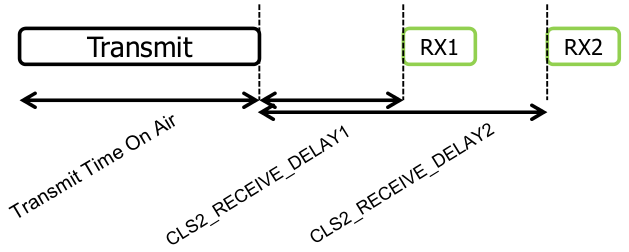
\includegraphics[width=0.4\textwidth]{img/lora_rx_windows.png}
  \end{figure}
\end{frame}

\begin{frame}[fragile]
  \frametitle{Class B end-devices}
  \begin{itemize}
		\item Class B end-devices are optimized for mobile and fixed battery-powered end-devices.
		\item They add a synchronized reception window called ``ping slot''
		\begin{itemize}
			\item Synchronization requires beacons;
			\item Devices selects randomly a ping slot at each beacon to avoid collisions.
		\end{itemize}
	\end{itemize}
	\begin{figure}
		\centering
		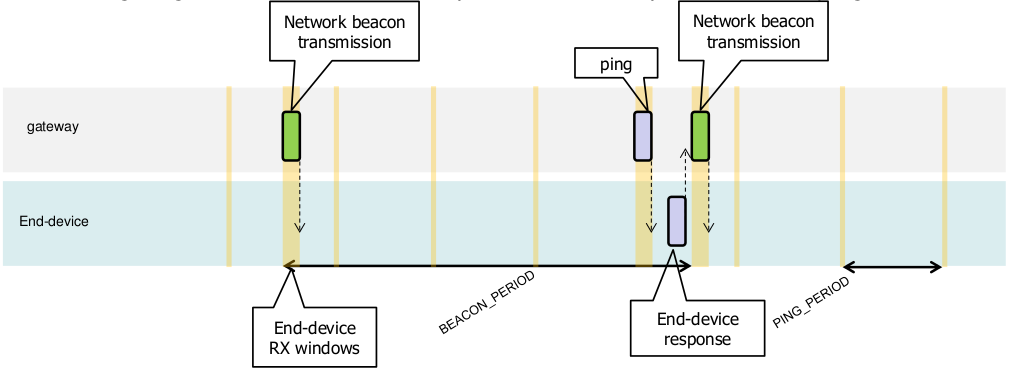
\includegraphics[width=0.8\textwidth]{img/loraBeacon.png}
	\end{figure}
\end{frame}

\begin{frame}[fragile]
  \frametitle{Class B end-devices}
  \begin{itemize}
		\item All end-devices start and join the network as end-devices of Class A.
		\item The end-device application can then decide to switch to Class B.
		\item The end-device waits a beacon and selects a ping slot of 30 ms from the 4096 available in a beacon interval.
		\item When the mote is far from BS the duration is extended, if beacon is not received the device tries to mantain the synchronization for 2 hours after that it returns to class A
  \end{itemize}
\end{frame}

\begin{frame}[fragile]
	\frametitle{Class C end-devices}
	\begin{itemize}
		\item This mode is used when there are no need for energy awareness and there's no need to minimize reception time.
		\item Class C end-devices cannot implement Class B option.
		\item These devices will listen with RX2 windows parameters as often as possible.
	\end{itemize}
	\begin{figure}
		\centering
		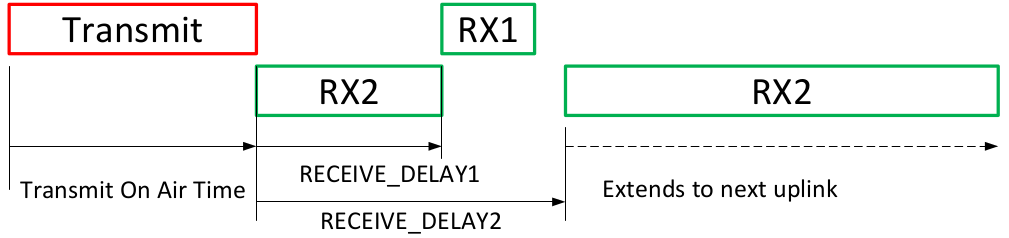
\includegraphics[width=0.8\textwidth]{img/loraClassC.png}
	\end{figure}
\end{frame}


\begin{frame}[fragile]
  \frametitle{LoRa secure communications - 1}
  In order to partecipate in a LoRa network an end device first has to be personalized and then activated.
  Activation of an end device can be achieved in two ways:
  \begin{itemize}
    \item OTAA (over-the-air activation) when an end device is deployed or reset;
    \item APB (activation by personalization) one-step personalization and activation.
  \end{itemize}
\end{frame}

\begin{frame}[fragile]
  \frametitle{LoRa secure communications - 2}
  During activation the end device holds the following informations:
  \begin{itemize}
      \item \textbf{DevAddr:} device ID of 32 bits that uniquely identifies the end device.
      \item \textbf{AppEUI:} globally unique application ID that uniquely identifies the application provider of the end device.
      \item \textbf{NwkSKey:} device-specific network session key, ensures data integrity and os used to encrypt/decrypt MAC data messages payload
      \item \textbf{AppSKey:} device-specific application session key, used to encrypt and decrypt the payload field of application-specific data messages.
  \end{itemize}
\end{frame}


\begin{frame}[fragile]
  \frametitle{LoRa secure communications - OTAA}
 \begin{figure}
  \centering
  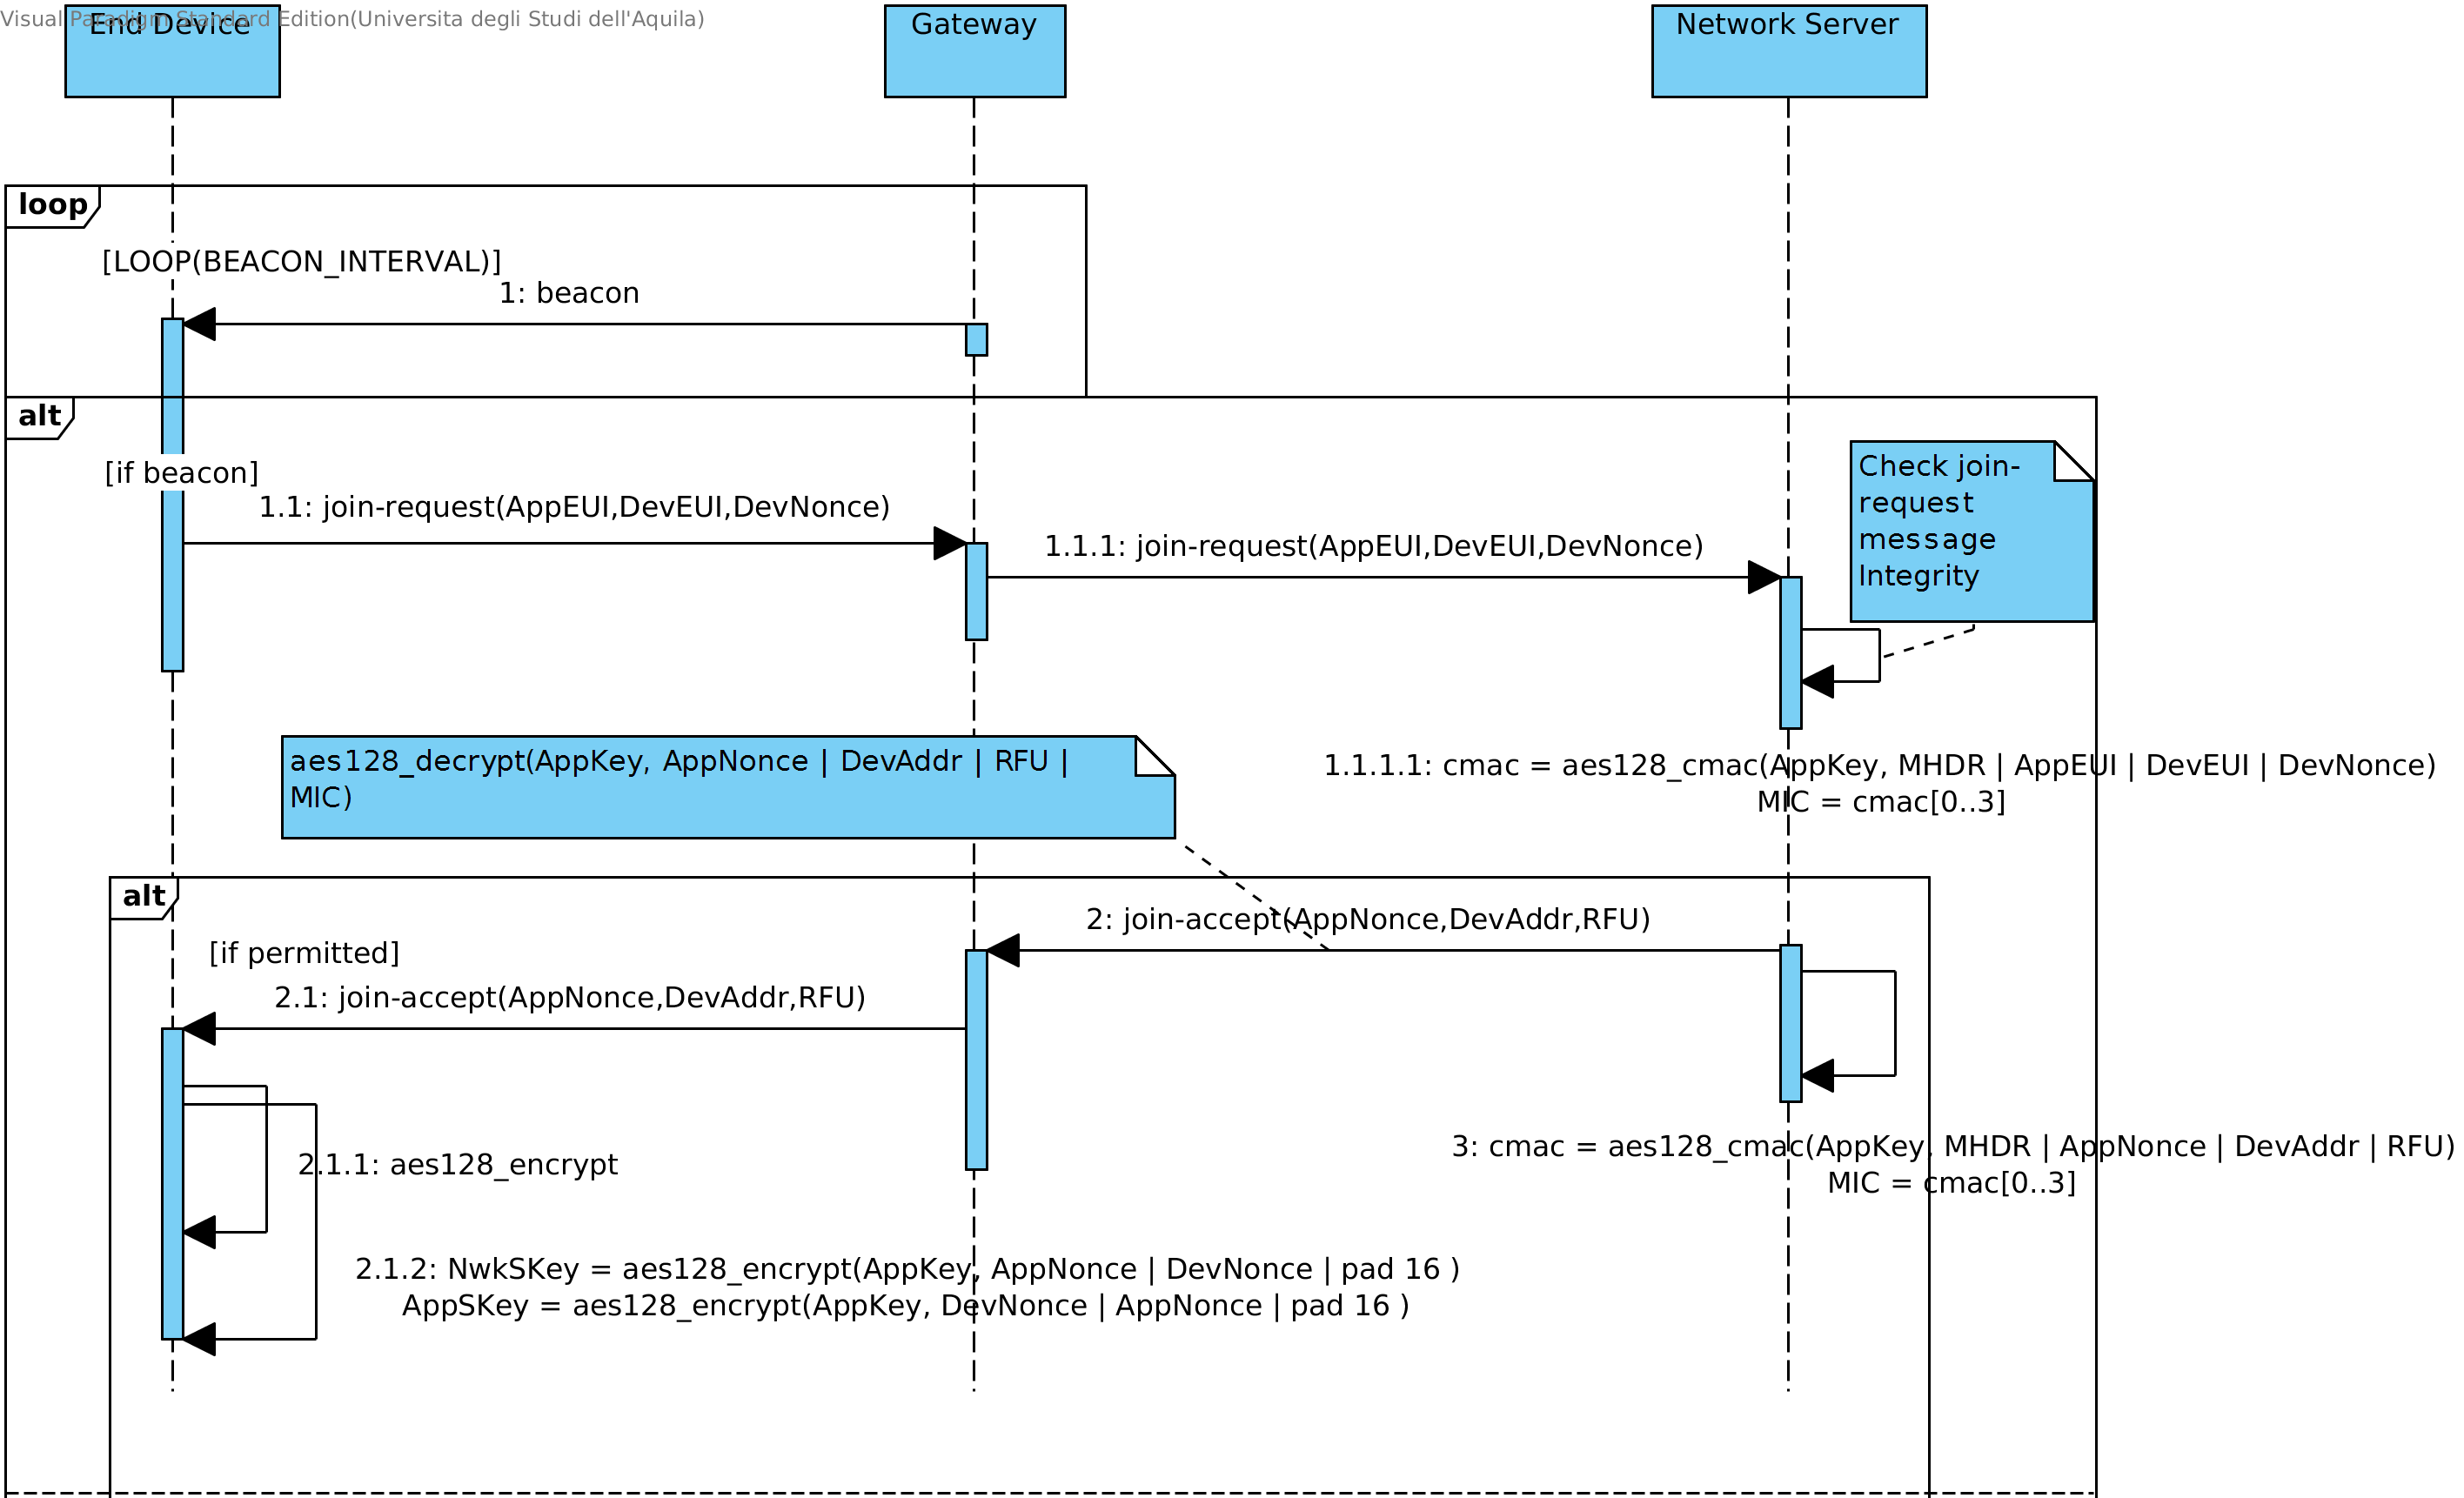
\includegraphics[width=0.9\textwidth]{img/lora_secure.png}
  \end{figure}
\end{frame}

\begin{frame}[fragile]
  \frametitle{LoRa mobility}
  LoRa network data rates are:
 \begin{itemize}
  \item Network controlled for fixed devices by means of using ADR bit in the PHY payload of data messages:
  \begin{itemize}
    \item If is set, the network will control the data rate of the end device through the appropriate MAC commands
    \item If is cleared, the network will not attempt to control the data rate of the end device independently of the received signal quality
  \end{itemize}
  \item default for mobile end-devices.
\begin{figure}
  \centering
  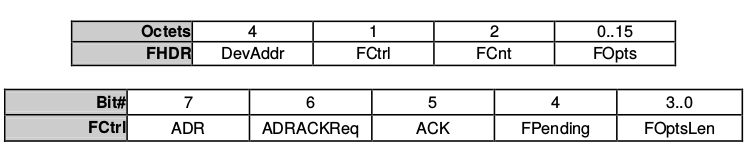
\includegraphics[width=0.9\textwidth]{img/PHYpayload.png}
  \end{figure}
 \end{itemize}
\end{frame}

\begin{frame}[fragile]
  \frametitle{LoRa mobility 2}
  LoRa modes (868Mhz band):
\begin{figure}
  \centering
  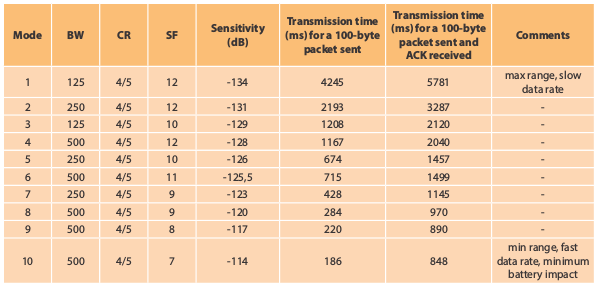
\includegraphics[width=0.9\textwidth]{img/LoRamode.png}
  \caption{SX1272 module modes}
 \end{figure}

\end{frame}


\begin{frame}[fragile]
  \frametitle{LoRa localization}
  All gateways send their beacon at exactly the same point in time:
  \begin{itemize}
    \item on first 15 bytes there are no visible on-air collisions 
    \item wrt the optional part , device within the proximity of more than one
	  gateway will still be able to decode the strongest beacon with high probability
  \end{itemize}
  \begin{figure}
  \centering
  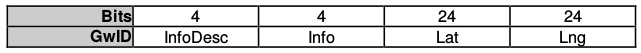
\includegraphics[width=0.9\textwidth]{img/optional.png}
  \caption{Beacon optional part}
 \end{figure}
  

\end{frame}

\begin{frame}[fragile]
  \frametitle{LoRa conclusions 1}
  For what applications is LoRa a good option?
  \begin{itemize}
    \item solar or mains-powered nodes transmitting every 10 or 15 minutes in networks with low or medium number of nodes
    \item very wide networks, with long-range links (Up to 22km, Sensitivity -134dBm) 
  \end{itemize}
  
\end{frame}
  
 \begin{frame}[fragile]
  \frametitle{LoRa conclusions 2}
  For what applications is NOT LoRa a good option?
  \begin{itemize}
    \item projects which require high data-rate and/or very frequent transmissions (e.g., each 10 seconds)
    \item including receipt of ACK message, mode 10 (the fastest), takes twice the time of XBee (<200ms)
    \item due to low data-rates OTA re-programming is not easily achieved (3G, GPRS may be better choiches)
  \end{itemize}
 
\end{frame}

